\documentclass{article}

\usepackage{graphicx}
\usepackage{tikz}
\usepackage{tikzsymbols}
\usetikzlibrary{calc,patterns,shapes.geometric}
\pagestyle{empty}
\usepackage[margin=0pt]{geometry}
\geometry{papersize={14in,12in}}

\def\centerarc[#1](#2)(#3:#4:#5){\draw[#1] ($(#2)+({#5*cos(#3)},{#5*sin(#3)})$) arc (#3:#4:#5);}

\begin{document}
	\begin{figure}
		\centering
		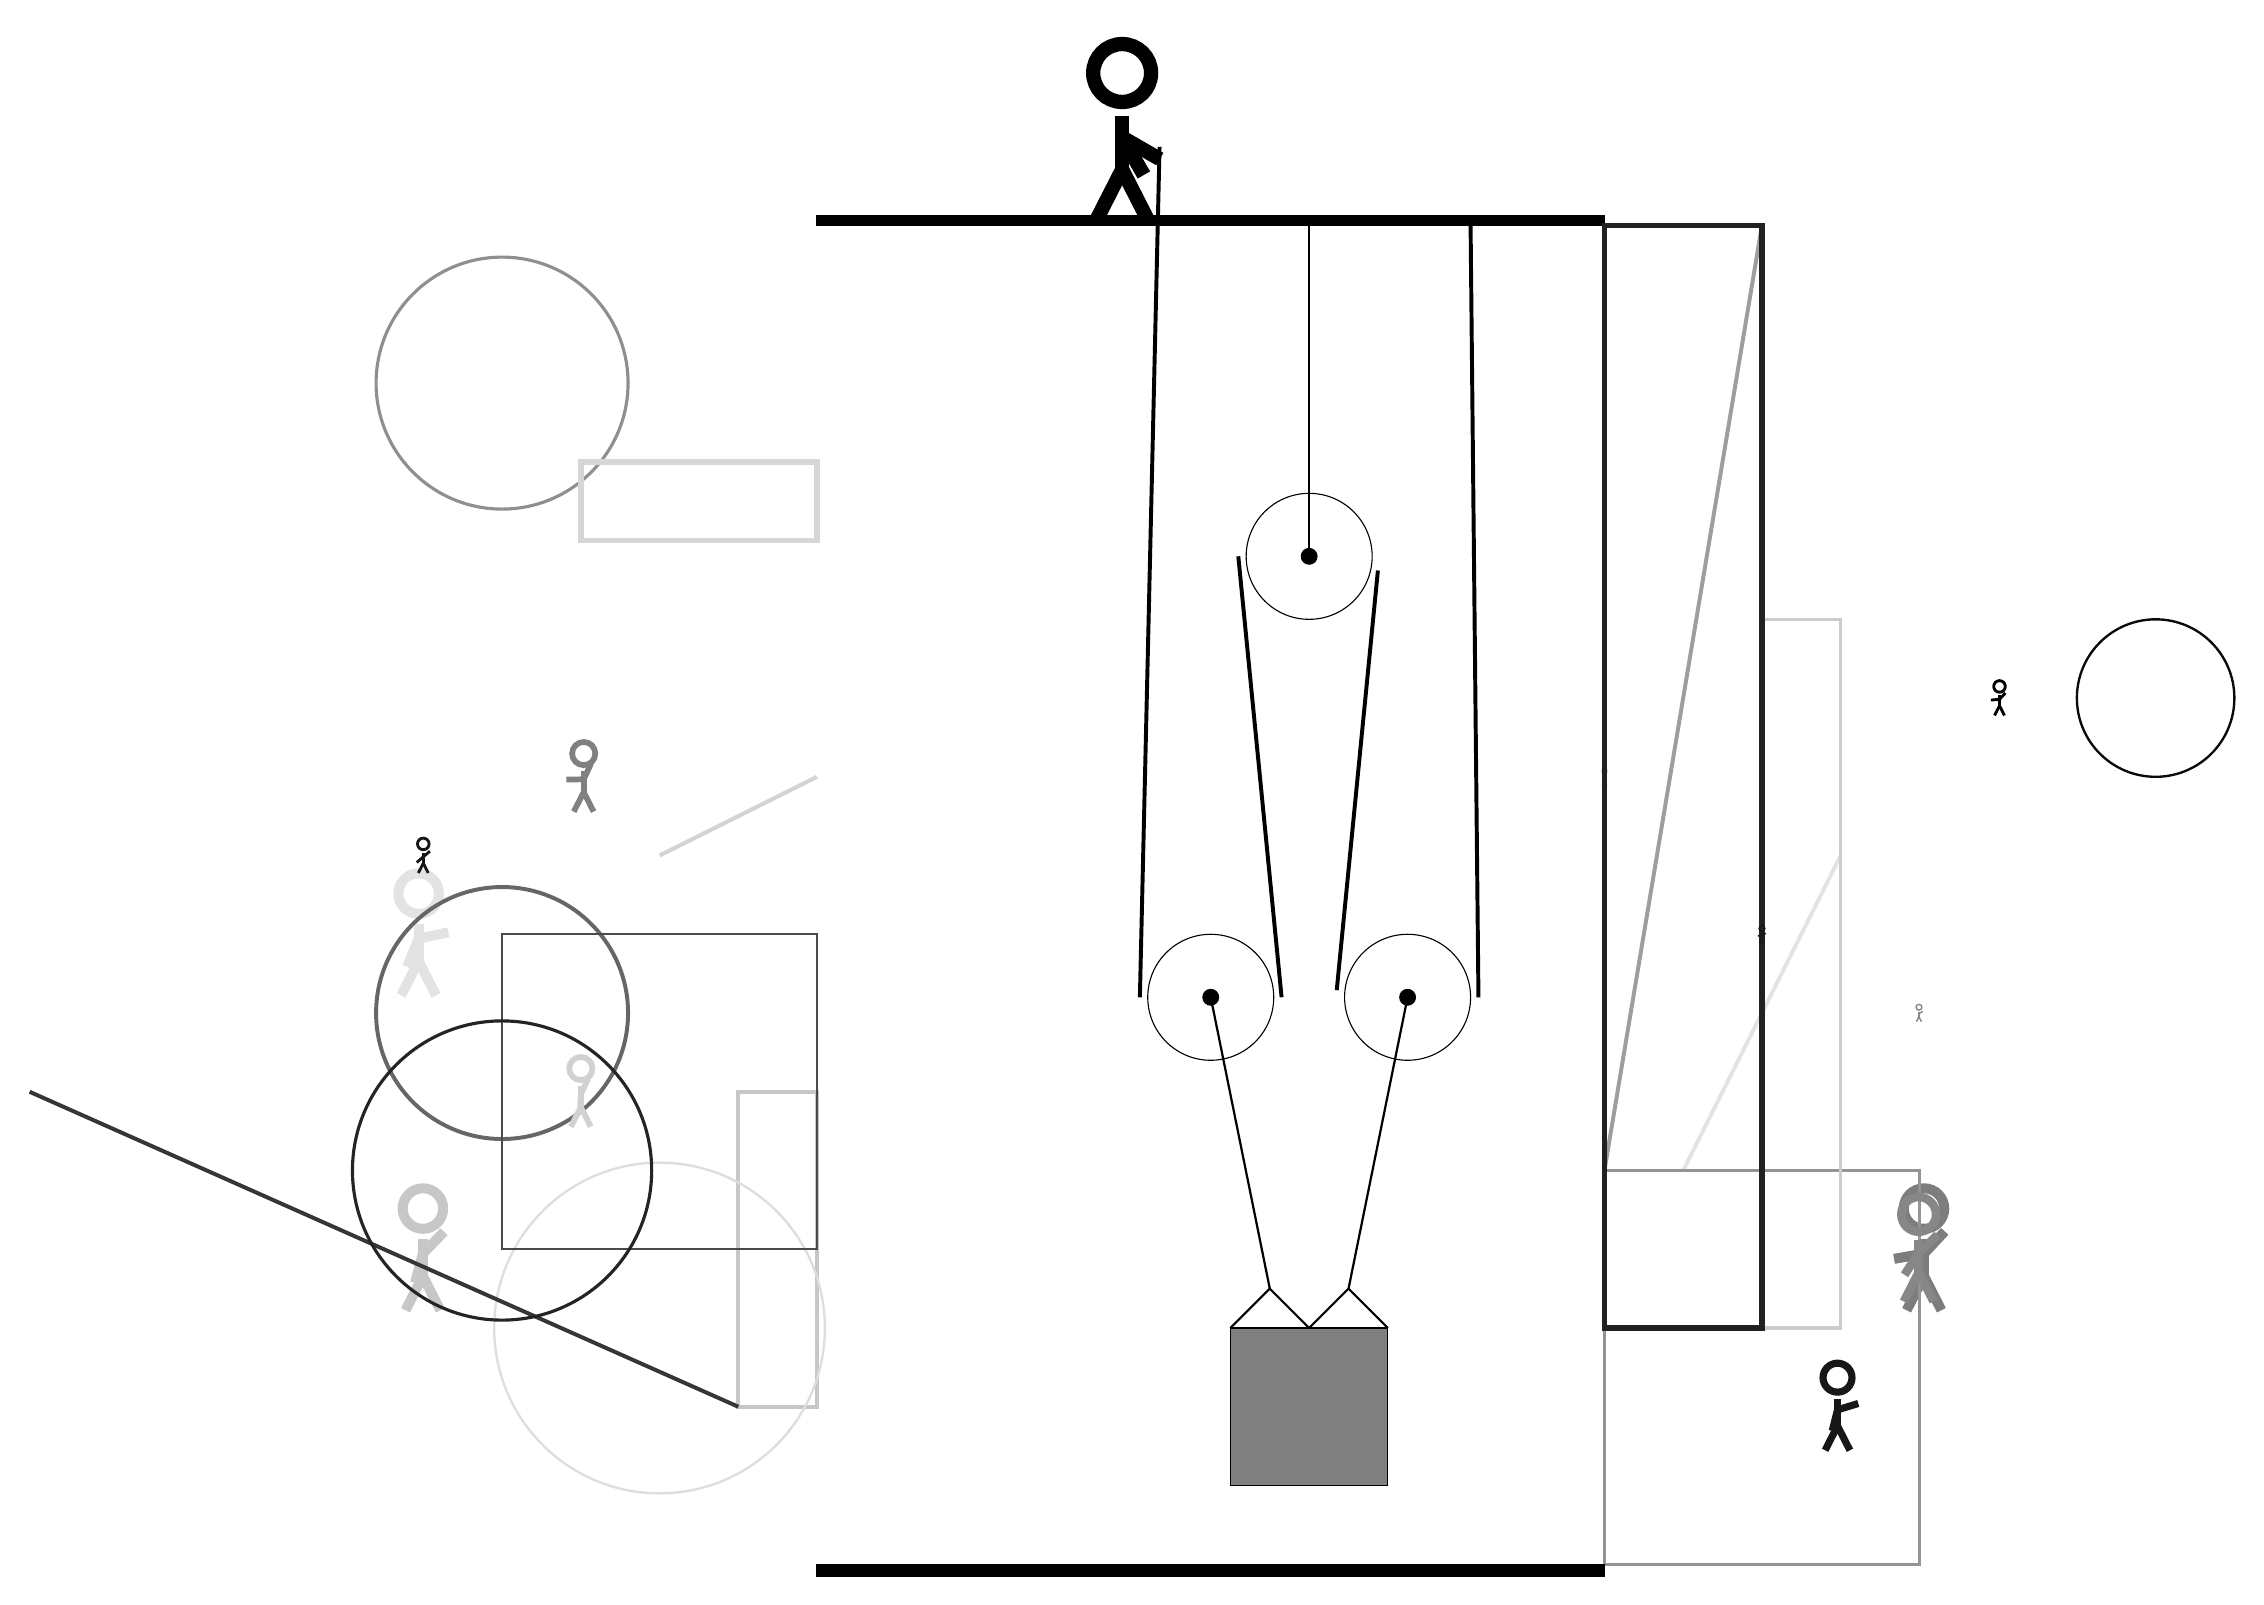
\begin{tikzpicture}
			%%%%% START %%%%%
			
			\draw[fill=black] (-4, 14) rectangle (6, 14.125);
			
			\draw[line width=0.5mm, color=black!38](6, 2) -- (8, 14);
			
			\draw [line width=0.4mm, color=black!44](-8, 12) circle (1.6);
			\node[line width=0.6mm, color=black!11] at (-9, 5) {\Strichmaxerl[7][68][12]};
			\node[line width=0.4mm, color=black!100] at (11, 8) {\Strichmaxerl[2][5][47]};
			\node[line width=0.2mm, color=black!18] at (6, 7) {\Strichmaxerl[1][88][84]};
			\node[line width=0.3mm, color=black!50] at (-7, 7) {\Strichmaxerl[4][1][65]};
			\node[line width=0.7mm, color=black!22] at (-9, 1) {\Strichmaxerl[7][75][46]};
			\node[line width=0.2mm, color=black!91] at (-9, 6) {\Strichmaxerl[2][41][40]};
			\draw [line width=0.5mm, color=black!60](-8, 4) circle (1.6);
			\draw[line width=0.5mm, color=black!22] (-5, -1) rectangle (-4, 3);
			
			\node[line width=0.3mm, color=black!91] at (9, -1) {\Strichmaxerl[5][76][17]};
			
			\node[line width=0.7mm, color=black!51] at (10, 1) {\Strichmaxerl[7][10][47]};
			\draw[line width=0.7mm, color=black!16] (-4, 11) rectangle (-7, 10);
			
			\draw[line width=0.5mm, color=black!11](7, 2) -- (9, 6);
			\draw [line width=0.3mm, color=black!13](-6, 0) circle (2.1);
			\draw[line width=0.5mm, color=black!79](-5, -1) -- (-14, 3);
			\draw[line width=0.3mm, color=black!71] (-4, 1) rectangle (-8, 5);
			\draw[line width=0.4mm, color=black!42] (6, -3) rectangle (10, 2);
			\draw [line width=0.3mm, color=black!96](13, 8) circle (1.0);
			\node[line width=0.7mm, color=black!18] at (-7, 3) {\Strichmaxerl[4][87][65]};
			\draw[line width=0.4mm, color=black!20] (8, 9) rectangle (9, 0);
			
			\draw [line width=0.4mm, color=black!86](-8, 2) circle (1.9);
			\draw[line width=0.5mm, color=black!17](-4, 7) -- (-6, 6);
			\draw [line width=0.4mm, color=black!94](10, -1) circle (0.0);
			\node[line width=0.2mm, color=black!47] at (10, 1) {\Strichmaxerl[6][57][44]};
			\draw[line width=0.7mm, color=black!87] (8, 14) rectangle (6, 0);
			\node[line width=0.7mm, color=black!47] at (10, 4) {\Strichmaxerl[1][82][31]};
			\node[line width=0.2mm, color=black!90] at (8, 5) {\Strichmaxerl[1][16][20]};
			
			\draw (1, 4.2) circle (0.8);
			\draw[fill=black] (1, 4.2) circle (0.1);
			
			\draw (2.25, 9.8) circle (0.8);
			\draw[fill=black] (2.25, 9.8) circle (0.1);
			\draw[thick] (2.25, 9.8) -- (2.25, 14);
			
			\draw (3.5, 4.2) circle (0.8);
			\draw[fill=black] (3.5, 4.2) circle (0.1);
			
			\draw[thick] (3.5, 4.2) -- (2.75, 0.5);
			\draw[thick] (1, 4.2) -- (1.75, 0.5);
			\draw[thick]  (1.25, 0) -- (1.75, 0.5) -- (2.25, 0);
			\draw[thick]  (2.25, 0) -- (2.75, 0.5) -- (3.25, 0);
			\draw[fill=black!50] (1.25, 0) rectangle (3.25, -2);
			
			\draw[line width=0.5mm] (0.35, 15) --  (0.1, 4.2);
			\centerarc[line width=0.5mm](1, 4.2)(180:360:0.9);
			\draw[line width=0.5mm] (1.9, 4.2) -- (1.35, 9.8);
			\centerarc[line width=0.5mm](2.25, 9.8)(-20:180:0.9);
			\draw[line width=0.5mm](3.123, 9.62) -- (2.6, 4.29);
			\centerarc[line width=0.5mm](3.5, 4.2)(160:360:0.9);
			\draw[line width=0.5mm](4.4, 4.2) -- (4.3, 14);
			
			\node at (-0.07, 15.2) {\Strichmaxerl[10][120][-30]};
			
			\draw[fill=black] (-4, -3) rectangle (6, -3.15);
			
			%%%%% END %%%%%
		\end{tikzpicture}
	\end{figure}	
\end{document}